\documentclass[10pt,twocolumn]{article}

% use the oxycomps style file
\usepackage{oxycomps}

% usage: \fixme[comments describing issue]{text to be fixed}
% define \fixme as not doing anything special
\newcommand{\fixme}[2][]{#2}
% overwrite it so it shows up as red
\renewcommand{\fixme}[2][]{\textcolor{red}{#2}}
% overwrite it again so related text shows as footnotes
%\renewcommand{\fixme}[2][]{\textcolor{red}{#2\footnote{#1}}}

% read references.bib for the bibtex data
\bibliography{references}

% include metadata in the generated pdf file
\pdfinfo{
    /Title (GitHub Tutorial)
    /Author (Julianne Yotov)
}

% set the title and author information
\title{GitHub Tutorial}
\author{Julianne Yotov}
\affiliation{Occidental College}
\email{jyotov@oxy.edu}

\begin{document}

\maketitle

\section{Introduction}

Computer programming is often a collaborative effort, so it is important to be able to store code and share it with others. A relatively straightforward and widely utilized way to do this is through GitHub, a user-friendly platform for developers to do just that. Git is the software system that GitHub uses, and it is known as a version control system, which will be discussed in greater detail.

\section{Getting Started}

GitHub can be operated through a desktop application, such as GitHub Desktop or Gitkraken, through the command line, or purely through the website. This tutorial will focus on using GitHub on a desktop application or on the command line. If you are new to GitHub or appreciate a more visual working environment, GitHub Desktop is a great option. To download, go to \url{https://desktop.github.com/} and follow the instructions for your operating system. If you would like to work with the command line interface, open the terminal.

\section{Introduction to Repositories}

\textit{Repositories} are used to store files for easy viewing and updating, and they can be shared with multiple people. They can be thought of as similar to folders on Google Drive, which are often used for group projects. 

\subsection{Creating Repositories}

To create a brand new repository on GitHub Desktop, simply click “Create a New Repository on your Hard Drive”. This will create a repository only on your machine, and you can later choose to publish it to github.com in order to collaborate on it with others. It is also helpful to check the “Initialize this repository with a README” option. A READM.md (markdown) file will allow you to write information that other people may need to understand your project. On the command line, you can create a new repository with the \texttt{git init} command.

\subsection{Cloning Repositories}

You can also \textit{clone} an existing repository, which means copying it from GitHub onto your local machine. On GitHub Desktop, click on “Clone a Repository from the Internet”. Typically, you should then type in the GitHub username and repository name: username/repository-name. Keep in mind that you can clone your own repository as well. On the command line, type \texttt{git clone} followed by the URL.

\subsection{Version Control}

As mentioned in the Introduction, Git is a version control system. This means that changes that are made to files are recorded, so that previous versions can be accessed at any time. This is similar to the version history in Google Docs and Microsoft Word that allows you to see previous versions of your document. You can click on “History” in GitHub Desktop to see all the changes that have been made. Now that you have created a new repository or cloned an existing one, you need to learn how to make changes to files and "save" them. 

\subsection{Working on Repositories}

On GitHub Desktop, you can open the repository in an external editor, which can be selected in Preferences. As shown in Figure 1, right-clicking on the repository will allow you to open the repository in your external editor (such as PyCharm) or the terminal. If the repository is published to GitHub, you can also view it on the website. Working in an external editor will allow you to easily add files or work on existing ones. The next section will go over how these changes can then be saved to your repository.

\begin{figure}
    \centering
    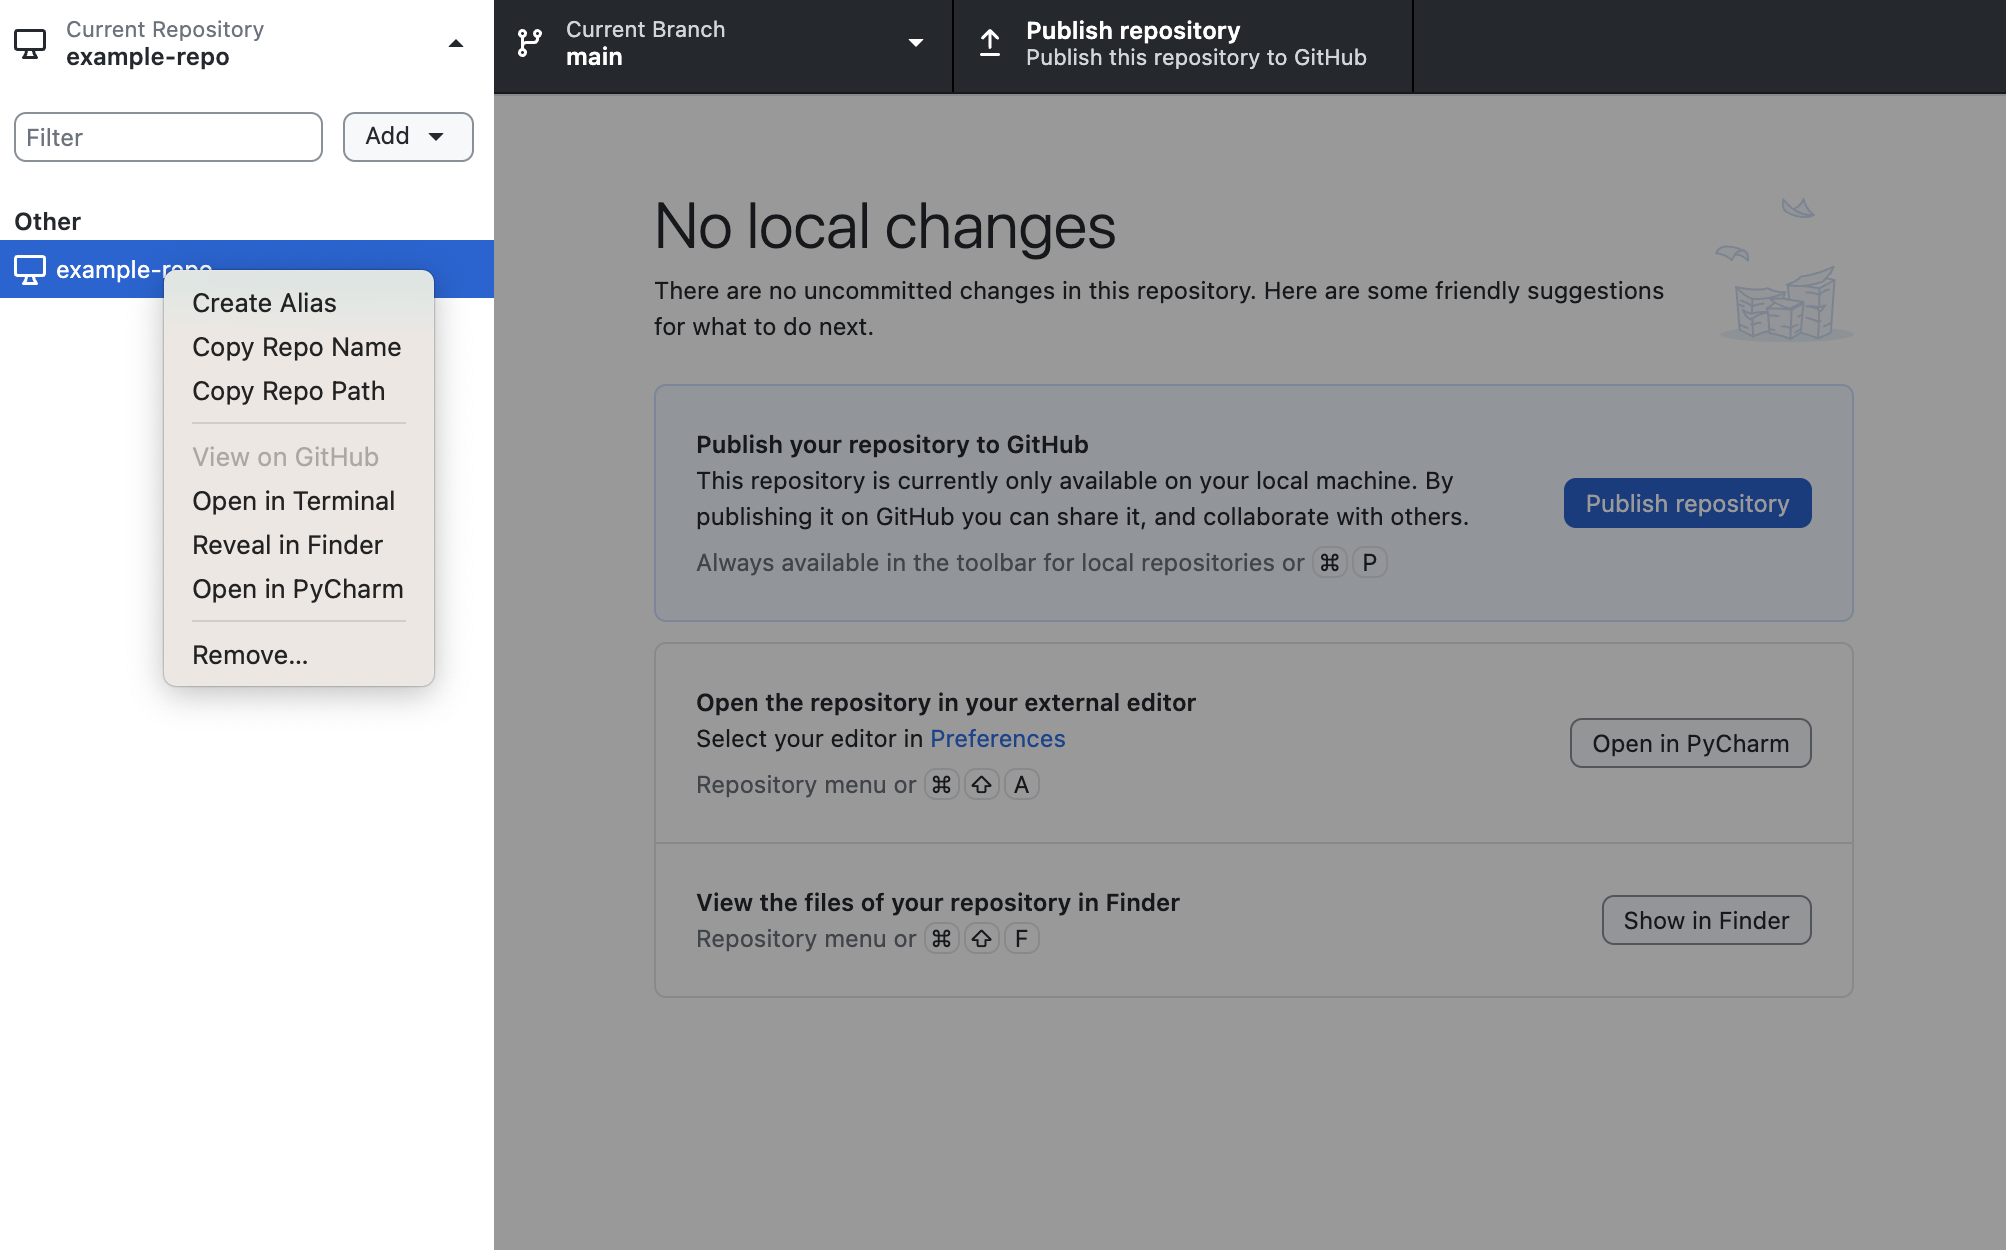
\includegraphics[width=.95\linewidth]{external_editor.png}
    \caption{
        Opening a repository in an external editor or the terminal
    }
    \label{fig:first-page}
\end{figure}

\section{Data Stores of Git and Transport Commands}

At this point, it is important to get a sense of where data can be stored on Git in order to introduce several commands that allow us to move information from one of these to another. \cite{DiveGit}


\begin{itemize}
    \item Working tree: As the name suggests, this is the area where you work. This is where the files currently on your computer are.
    \item Staging area (or index): This is the location of files and changes that are ready to be committed. This command allows for changes made to files to be recorded.
    \item Local repository: These are the repositories on individual computers that contain files that have been committed, along with their history.
    \item Remote repository: These are the repositories that are on a different computer and are accessible to everyone involved in that project. 
\end{itemize} 

\subsection{Working Tree to Staging Area: \texttt{add}}

In order to transport something from the working tree to the staging area, the \textit{add} command is used. This is an important intermediate step because it is a way to signal that a file is ready to be committed without actually doing so. Therefore, multiple files that may need to be committed at the same time can be added to the staging area first. On the command line, use the \texttt{git add} command followed by the file name, such as README.md. On GitHub Desktop, the “Add” button that appears when you click the “Current Repository” dropdown does not refer to this command. Instead, committing is equivalent to combining the \textit{add} and \textit{commit} commands, which is why the command line approach may be preferable in this case.

\subsection{Staging Area to Local Repository: \texttt{commit}}

The \textit{commit} command is used to record changes made to the files in your local repository. As previously discussed, you can open your repository in an external editor in GitHub Desktop and add files or change existing ones. These local changes will then be reflected in GitHub Desktop, which is where you can easily commit them. As an example, open your repository in an external editor and create a file containing something, such as \texttt{print('Hello, World!')}. This change will be noted in GitHub Desktop. You then will need to select the file(s) to commit and write a brief summary (ideally less than 50 characters) on the change that you made (if it doesn’t automatically fill it in). You can also add an optional description regarding the change for later reference. Then, you can click “Commit to main” to save the change. This process is shown in Figure 2. On the command line, simply use the command \texttt{git commit} to commit all files in the staging area. The command \texttt{git commit -m} followed by a message in quotes allows you to note the commit that is being made. 

\begin{figure}
    \centering
    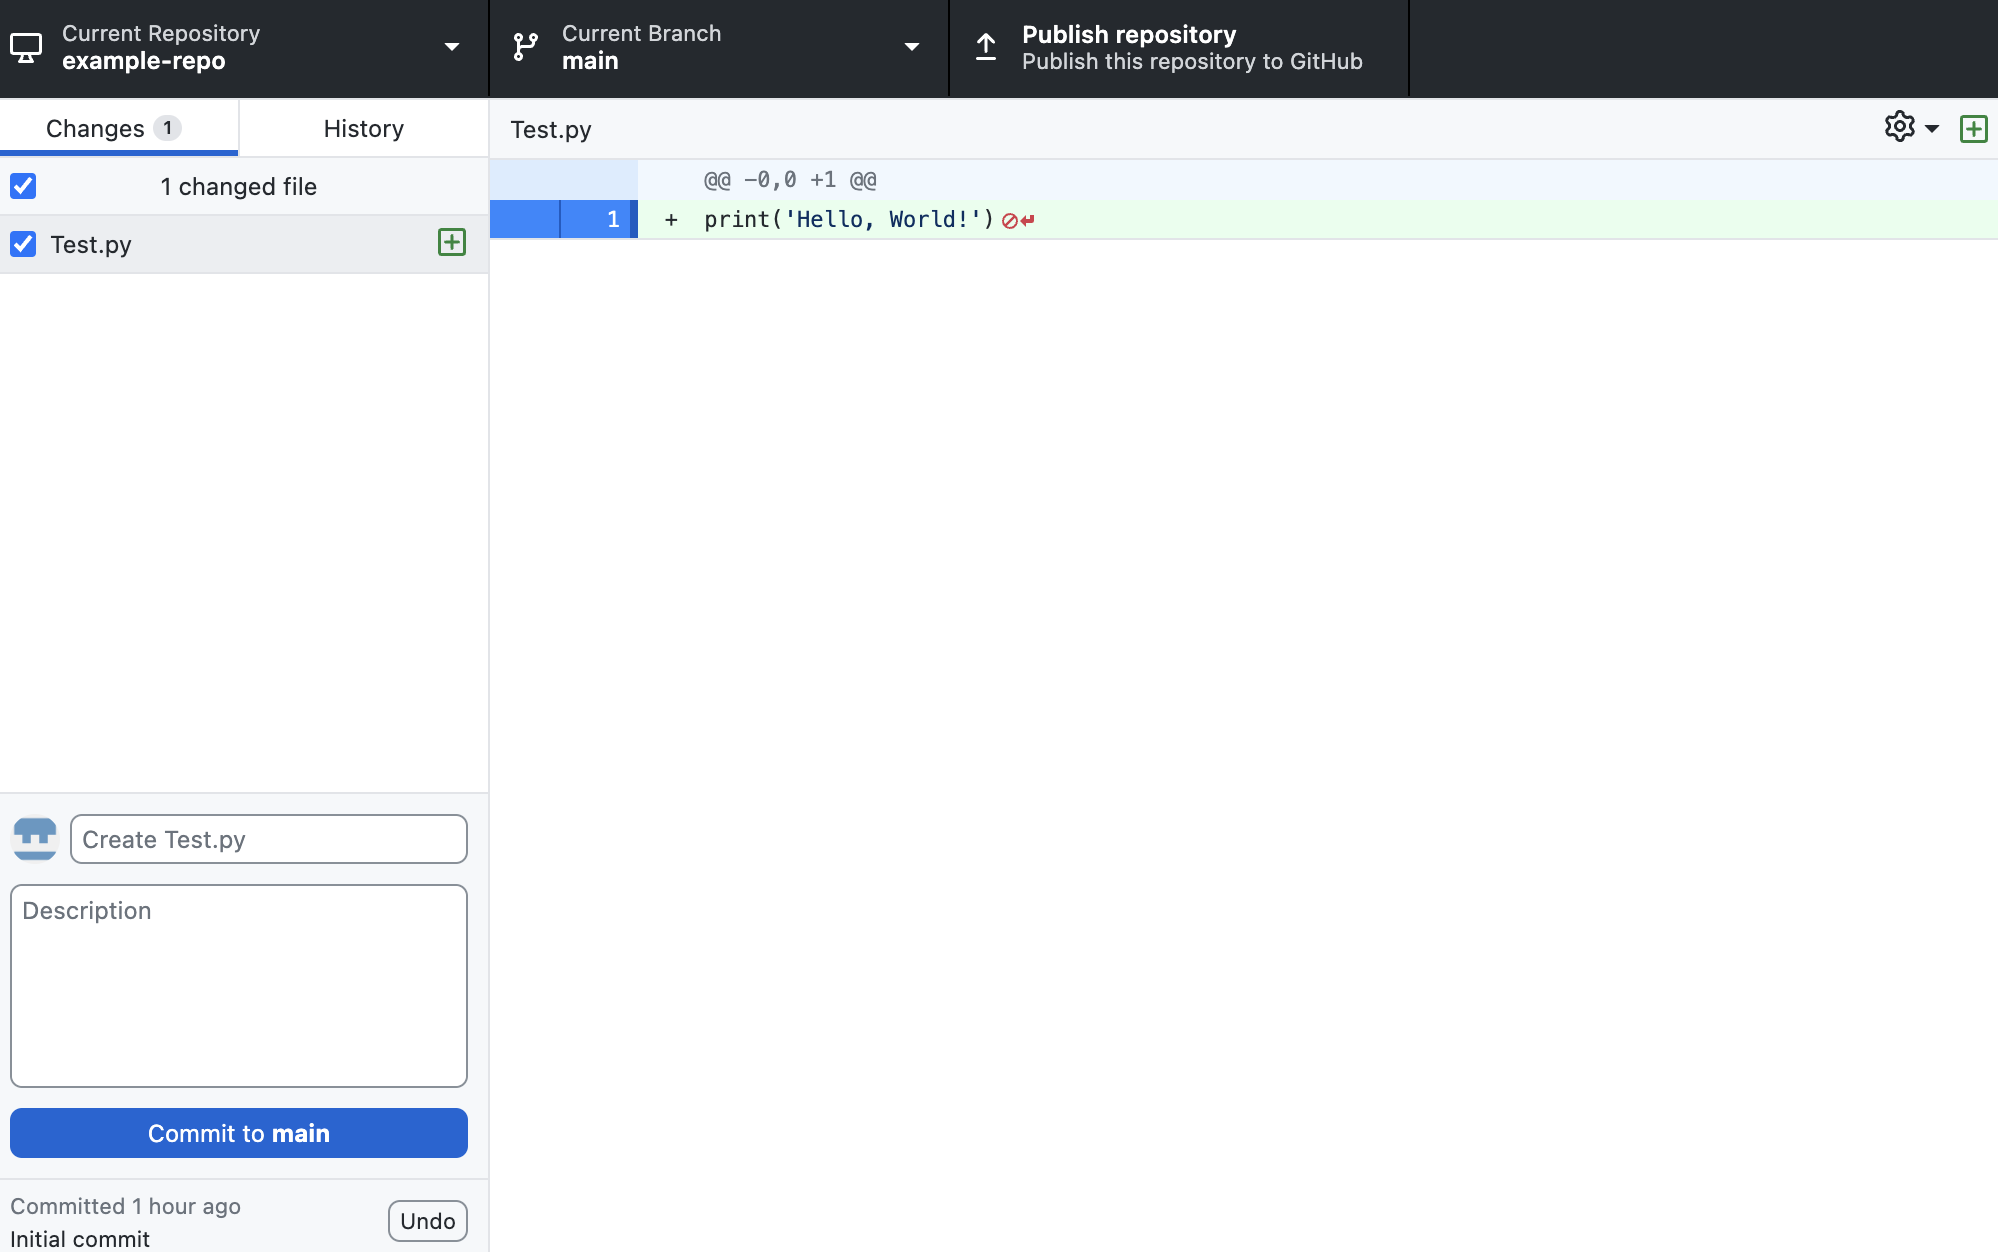
\includegraphics[width=.95\linewidth]{commit.png}
    \caption{
        Committing on GitHub Desktop
    }
    \label{fig:first-page}
\end{figure}

\subsection{Local Repository to Remote Repository: \texttt{push}}

The \textit{push} command is used to transport something from your local repository to a remote repository. As a simple example, let’s say we clone a repository, add a file, and commit the change. On GitHub Desktop, you will see a tab that says “Push origin”. Clicking this will update the remote repository to match the committed change in your local repository. On the command line, there are many different options, as outlined in \url{https://git-scm.com/docs/git-push#OPTIONS}. A common command is \texttt{git push}, which works if a remote repository already exists for that branch.

\subsection{Remote Repository to Local Repository: \texttt{pull}}

It is also possible to \textit{pull} something from a remote repository and transfer it to your local repository. In order to effectively discuss how and why to create a \textit{pull request}, it is necessary to discuss branches and merging.

\section{Branches and Merging}

A \textit{branch} in Git can be thought of as a container storing some changes. Creating a branch allows you to develop features, fix bugs, and experiment with the code. All repositories have a main branch, and you can create additional branches.

\subsection{Creating a Branch}

To create a new branch on GitHub Desktop, click on the "Current Branch" tab. You can then type in a name for this new branch and click "Create New Branch". On the command line, use \texttt{git branch} followed by the chosen name.

\subsection{Merging Two Branches}

Once you have created a new branch, you can make changes to existing files or create new ones. Once you do so, the contents of this new branch will no longer be up to date with the main branch. Eventually, you may want to ensure that the main branch reflects the changes you have made in the new branch. This is especially important if collaborating on a project with others; they will need to be able to see the work that you have done. GitHub is able to check if the new branch can be \textit{merged} with the main branch, which is a way of transferring the changes in the new branch to the main branch. Therefore, the main branch will reflect the changes made in the new branch. In GitHub Desktop, click on the main branch and then “Choose a branch to merge into \textbf{main}”. You will then be able to select the branch to be merged into the main branch. Eventually, the new branch can be deleted if it is no longer needed. On the command line, use \texttt{git checkout} and indicate the branch that the new branch will be merged into (typically the main branch). Then use \texttt{git merge}, followed by the name of this new branch.

\subsection{Merge Conflict}

It is not always possible to merge two (or more) branches. A \textit{merge conflict} occurs if the branches contain conflicting information. For example, if two people made different changes to the same line of a file and both attempt to merge their respective branches, such a conflict will occur. Similarly, if two branches contain files with the same name but different contents, or if one person deletes a file that another other person changes, the branches won’t be able to both be merged. This is why it is important to ensure that all members working on a project work on different parts. If one person wants to build upon another person’s work, they should wait for them to push their work to the remote repository and then create a pull request.

\subsection{Pull Request}

You will be given the option to create a pull request in GitHub Desktop if your branch is already published to GitHub. This will take you to GitHub, where you can create the pull request if the two branches can be merged. Alternatively, on the command line, \texttt{git pull origin main} will either clone the remote repository or transfer the changes from the remote repository to your local repository. 

\section{Stashes}

The stash command saves uncommitted changes for later use and removes them from the file. In GitHub Desktop, you can right-click on “x changed files” rather than committing the changes, followed by “Stash All Changes”. These changes can later be restored or deleted. This is particularly useful if you have made changes that you do not yet wish to commit. Additionally, if there is a merge conflict due to changes in your branch, you can stash the changes and recover them later (Figure 3).

\begin{figure}
    \centering
    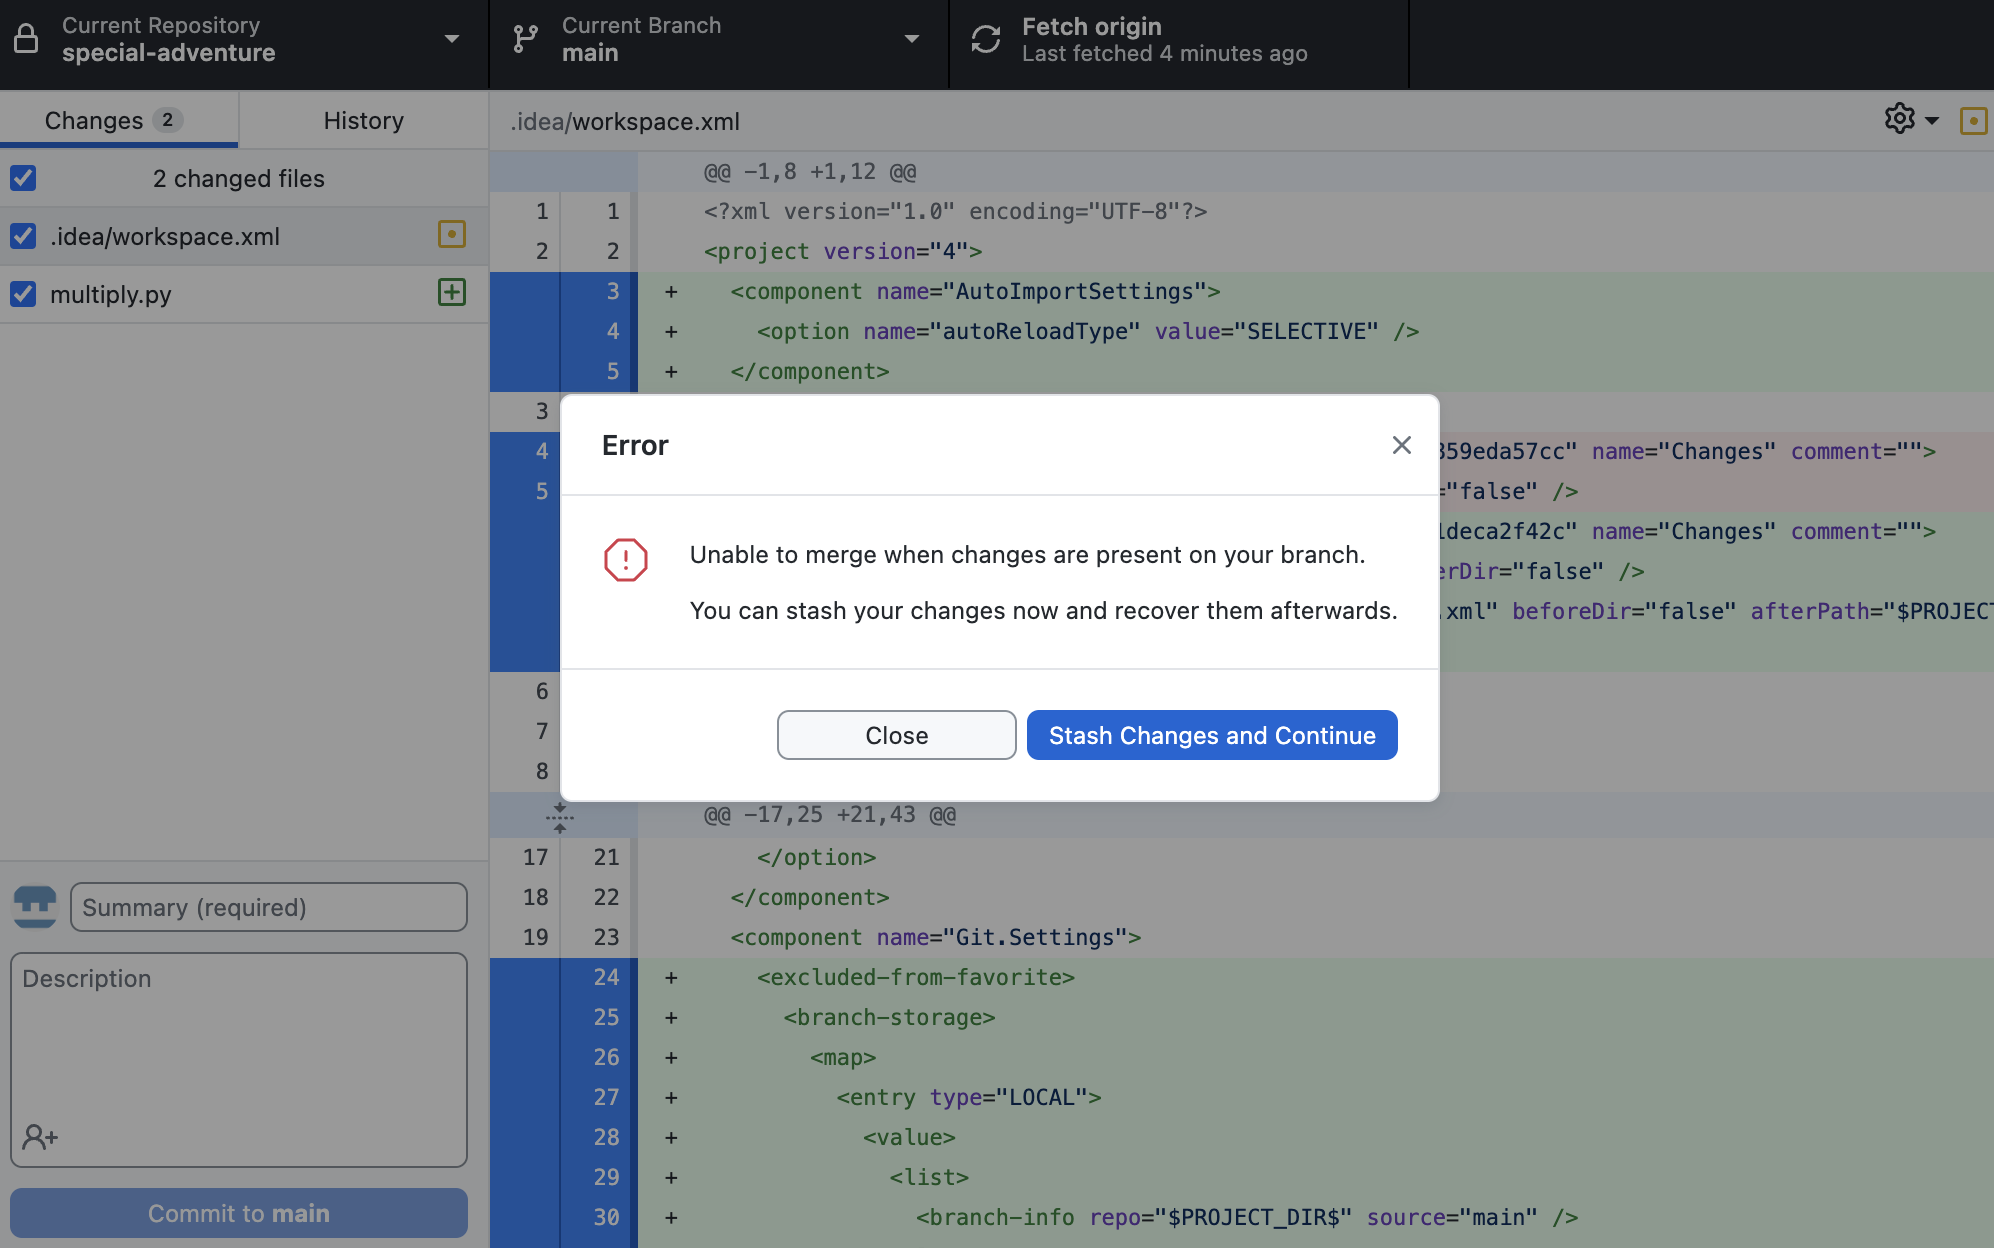
\includegraphics[width=.95\linewidth]{stashing.png}
    \caption{
        Stashing changes to avoid merge conflict
    }
    \label{fig:first-page}
\end{figure}


\section{Conclusion}

This tutorial covers some of the basics of GitHub, but there is still much more to learn and explore. A couple of great resources are: \url{https://git-scm.com/} \cite{GitHubDocs} and \url{https://docs.github.com/en} \cite{git}.

\printbibliography

\end{document}
